

\section{Введение}
Во время различных научных экспериментов часто возникает задача определить некоторую физическую величину при помощи измерительных приборов. При измерении  невозможно получить ее абсолютно точное значение, так как не существует идеальных измерительных инструментов и методов.

По этой причине, после произведённого измерения физической величины, нужно указать погрешность измерения.

На значение конкретного измерения влияют систематические и случайные погрешности. Их источниками могут являться сами измерительные приборы. Кроме того, погрешность может возникать из-за несовершенства методики измерения и промахов самого экспериментатора. 


\subsection{Задачи работы}

Таким образом, задачами данной работы являются:
\begin{enumerate}
    \item Освоить методику использования измерительного прибора для
многократного прямого измерения физической величины.
    \item Выполнить простейшую статистическую обработку серии
результатов наблюдений при прямых измерениях.

\end{enumerate}




\section{Основная часть}

\subsection{Теоретическая часть}
Для оценки погрешности измерения физическую величину необходимо измерить несколько раз. Таким образом, будет получена соответствующая выборка:


\begin{equation}
    x_1,x_2,x_3, ..., x_n
\end{equation}
Значения из выборки отличаются от истинного значения измеряемой физической величины. Это вызвано влиянием погрешностей на каждое единичное измерение.\\
Необходимо определить, что целесообразнее всего считать результатом измерения. В качестве оптимального значения измеряемой величины (то есть результата измерения) принимается среднее арифметическое.
\begin{equation}
    \overline{x}=\frac{x_1+x_2+...+x_n}{n}=\frac{1}{n}\sum_{i=1}^{n} x_i
\end{equation}
Приняв, что измеряемая величина равна среднему значению, можно производить дальнейший анализ полученных данных. Стоит убедиться в отсутствии дрейфа - изменением значений с течением времени.
Дальнейший анализ полученной выборки состоит в рассмотрении распределения результатов наблюдения с помощью гистограммы, графика зависимости или наблюдении результатов на числовой оси.\\
С помощью графика зависимости можно определить дисперсию распределения (среднюю квадратическую погрешность отдельного наблюдения). Кроме того, дисперсию можно найти по приближенной формуле (6):
\begin{equation}
    \sigma=\sqrt{\frac{1}{n-1}\sum_{i=1} (x_i-\overline{x})^2}
\end{equation}
Средняя квадратичная погрешность среднего связана с дисперсией следующей формулой:
\begin{equation}
    \sigma_{\overline{x}}=\frac{\sigma}{\sqrt{n}} ,
\end{equation}
где n - число измерений.
Интервал, внутрь которого с заданной вероятностью попадает истинное значение задаётся следующим выражением:
\begin{equation}
    x=\overline{x}\pm\sigma_{\overline{x}} ,
\end{equation}


\subsection{Эксперимент}
Лабораторная работа заключается в измерении  электронным частотомером ЧЗ-32 частоты следования импульсов.\\ От генератора сигналов на частотомер подается последовательность
прямоугольных импульсов, заданных параметров. Частота следования импульсов измеряется с помощью частотомера на двух
шкалах: грубой и точной. В качестве генератора импульсов используется
генератор Г5-15, а в качестве частотомера – Ч3—32.\\
Схема установки приведена на рис.~\ref{fig:Схема установки}. На рис.~\ref{fig:установка} представлена фотография установки, сделанная во время проведения лабораторной работы.

\begin{figure}[H]
\centering
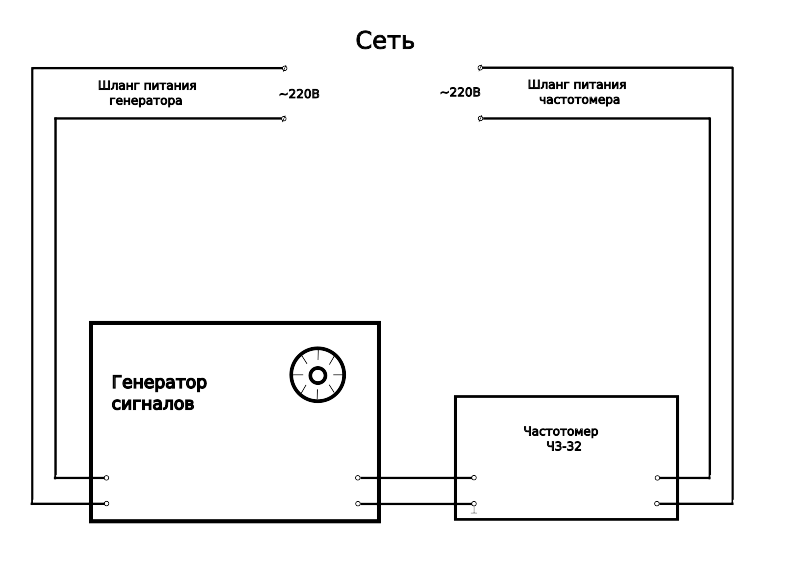
\includegraphics[width=0.8\textwidth]{Схема установки}
\caption{Схема установки}
\label{fig:Схема установки}
\end{figure}



\begin{figure}[H]
\centering
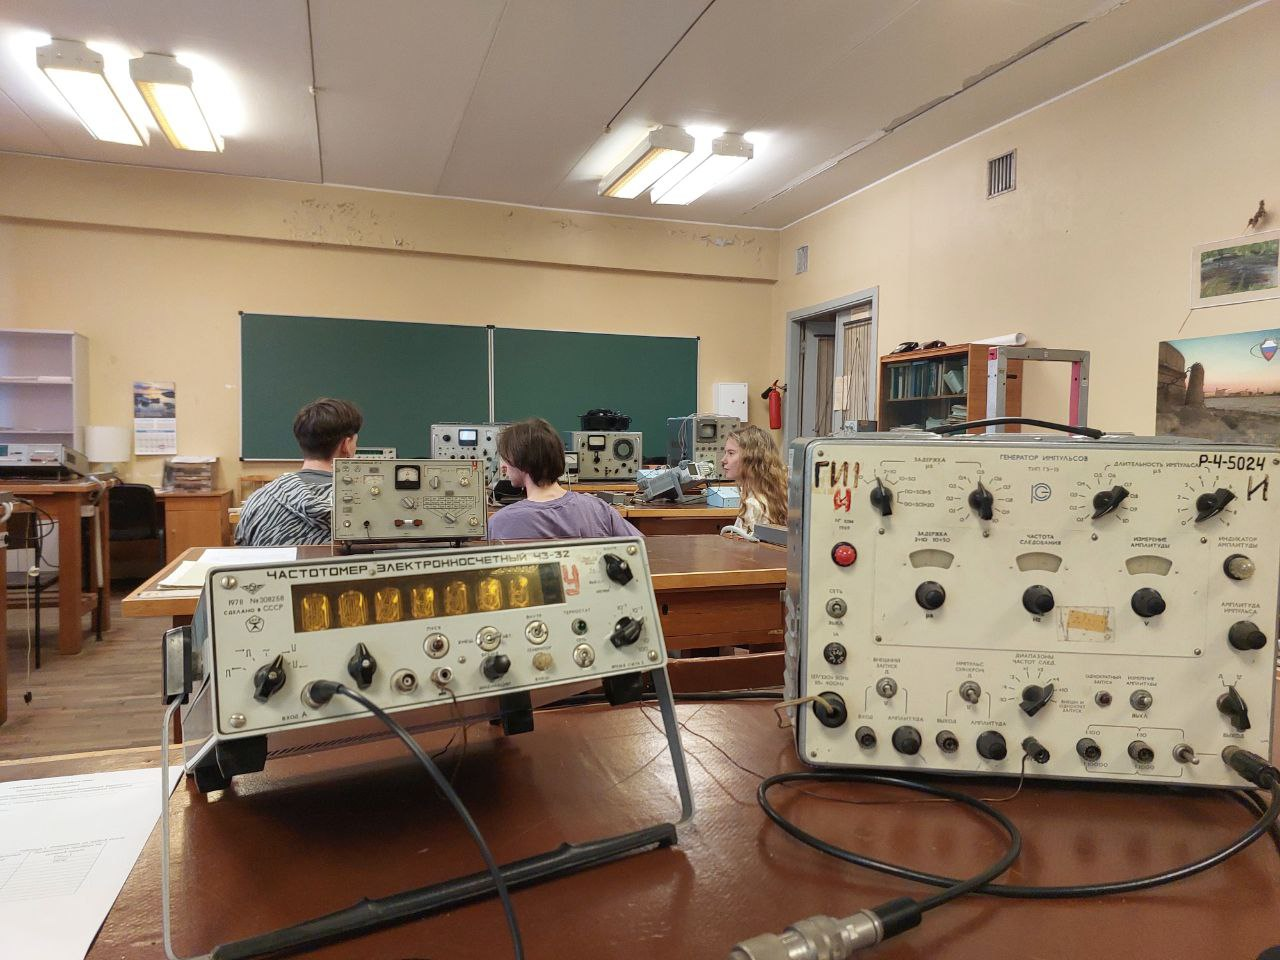
\includegraphics[width=0.8\textwidth]{Установка.jpg}
\caption{Установка}
\label{fig:установка}
\end{figure}

\subsection{Обработка данных и обсуждение результатов}
Вычисление погрешности прибора $\Delta f$ производится по следующим формулам:
\begin{equation}
   \gamma_f=  \frac{\Delta f}{f_x}*100\%
   \label{eq:6}
\end{equation}
\begin{equation}
 \gamma_f=\pm(\gamma_0+\frac{1}{(f_x*T)})*100,
    \label{eq:7}
 \end{equation}
 где $\gamma_f$ - относительная погрешность прибора, $\gamma_0$=$\pm$$5*10^{-7}$, T=0.1 с на грубой шкале, T=1 с на точной шкале.\\
 На грубой шкале было произведено 10 измерений, результаты представлены в таблице ~\ref{tabl:1}.

\begin{center}
\begin{table}[h!]
\centering
\caption{Измерения на грубой шкале}
\label{tabl:1}
\begin{tabular}{|c|c|c|c|c|}
\hline
\begin{minipage}{7mm}
    № п.п. 
\end{minipage}&
\begin{minipage}{5cm}
    Диапазон показаний использованной шкалы прибора
\end{minipage} &
\begin{minipage}{5cm}
    Результаты отдельных наблюдений ($f_i$)
\end{minipage} &
\begin{minipage}{5cm}
    Погрешность прибора на данной шкале ($\Delta f_{\text{приб}}$)
\end{minipage}\\
\hline
{}&кГц&кГц&кГц\\
\hline
1 &  0-10^5  &  4.56  &  0.0100 \\
2 &  0-10^5  &  4.54  &  0.0100 \\
3 &  0-10^5  &  4.54  &  0.0100 \\
4 &  0-10^5  &  4.56  &  0.0100 \\
5 & 0-10^5  &  4.56  &  0.0100 \\
6 & 0-10^5  &  4.56  &  0.0100 \\
7 & 0-10^5  &  4.58  &  0.0100 \\
8 & 0-10^5  &  4.56  &  0.0100 \\
9 & 0-10^5  &  4.58  &  0.0100 \\
10& 0-10^5  &  4.56  &  0.0100 \\
\hline
\end{tabular}
\end{table}
\end{center}
Так же было получено $\overline{f}$=4.56 кГц.\\

На точной шкале погрешность прибора $\Delta f_{\text{приб}}$ составила 0.001002 кГц.
Результаты 43 измерений, произведенных на точной шкале представлены в таблице ~\ref{tabl:2}.
\begin{center}
\begin{table}[H]
\centering
\caption{Измерения на точной шкале}
\label{tabl:2}
\begin{tabular}{|c|c|c|c|c|}
\hline
\begin{minipage}{7mm}
    № п.п. 
\end{minipage}&
\begin{minipage}{5cm}
    Результаты отдельных наблюдений ($f_i$)
\end{minipage} &
\begin{minipage}{5cm}
    Случайные отклонения от среднего d_i=$f_i-\overline{f}$
\end{minipage} &
\begin{minipage}{5cm}
   d_i^2=($f_i-$$\overline{f}$)^2
\end{minipage}\\
\hline
{}&кГц&кГц&кГц^2\\
\hline

1  &    4.542  &  0.001 & 0.000001 \\
2  &    4.540  &  -0.001 & 0.000001 \\
3 &  4.538  &  -0.003 & 0.000009 \\
4 &  4.542  &   0.001 & 0.000001 \\
5 &  4.542  &  0.001 & 0.000001 \\
6 &  4.542  &  0.001 & 0.000001 \\
7 &  4.540  &  -0.001 & 0.000001 \\
8 &  4.542  &  0.001 & 0.000001 \\
9 &  4.542  &  0.001 & 0.000001 \\
10 &  4.542  &  0.001 & 0.000001 \\
11 &  4.542  &  0.001 & 0.000001 \\
12 &  4.542  &  0.001 & 0.000001 \\
13 &  4.542  &  0.001 & 0.000001 \\
14 &  4.544  &  0.003 & 0.000009 \\
15 &  4.544  &  0.003 & 0.000009 \\
16 &  4.544  &  0.003 & 0.000009 \\
17 &  4.544  &  0.003 & 0.000009 \\
18 &  4.544  &  0.003 & 0.000009 \\
19 &  4.542  &  0.001 & 0.000001 \\
20 &  4.542  &  0.001 & 0.000001 \\
21 &  4.540  &  -0.001 & 0.000001 \\
22 &  4.540  &  -0.001 & 0.000001 \\
23 &  4.542  &  0.001 & 0.000001 \\
24 &  4.540  &  -0.001 & 0.000001 \\
25 &  4.542  &  0.001 & 0.000001 \\
26 &  4.540  &  -0.001 & 0.000001 \\
27 &  4.540  &  -0.001 & 0.000001 \\
28 &  4.540  &  -0.001 & 0.000001 \\
29 &  4.538  &  -0.003 & 0.000009 \\
30 &  4.540  &  -0.001 & 0.000001 \\
31 &  4.540  &  -0.001 & 0.000001 \\
32 &  4.540  &  -0.001 & 0.000001 \\
33 &  4.540  &  -0.001 & 0.000001 \\
34 &  4.540  &  -0.001 & 0.000001 \\
35 &  4.538  &  -0.003 & 0.000009 \\
36 &  4.540  &  -0.001 & 0.000001 \\
37 &  4.538  &  -0.003 & 0.000009 \\
38 &  4.540  &  -0.001 & 0.000001 \\
\hline
\end{tabular}
\end{table}
\end{center}
\begin{center}
\begin{table}[H]
\centering

\label{tabl:11}
\begin{tabular}{|c|c|c|c|c|}
\hline
\begin{minipage}{7mm}
    № п.п. 
\end{minipage}&
\begin{minipage}{5cm}
    Результаты отдельных наблюдений ($f_i$)
\end{minipage} &
\begin{minipage}{5cm}
    Случайные отклонения от среднего d_i=$f_i-\overline{f}$
\end{minipage} &
\begin{minipage}{5cm}
    Погрешность прибора на данной шкале d_i^2=($f_i-$$\overline{f}$)^2
\end{minipage}\\
\hline
{}&кГц&кГц&кГц^2\\
\hline
39 &  4.538  &  -0.003 & 0.000009 \\
40 &  4.538  &  -0.003 & 0.000009 \\
41 &  4.538  &  -0.003 & 0.000009 \\
42 &  4.542  &  0.001 & 0.000001 \\
43 &  4.541  &  0 & 0.000000 \\
\hline
   &  $\overline{f}$=4.541 & d_i=-0.006 & $d_i^2=0.000138$\\
\hline
\end{tabular}
\end{table}
\end{center}
\subsubsection{Исходный код}
Приведём описание работы программы "Precise measure", написанной на C++, предназначенной для обработки результатов, полученных в ходе измерений на точной шкале. 
\parФункция inputdata() нужна для ввода данных из файла "Precise measurements.csv" \\и сохранения их в массив arr1.
\parФункция arithmetic\underline{ }mean() вычисляет среднее арифметическое значение массива arr1 с округлением до четырёх значащих цифр.
\parФункция relative\underline{ }error() рассчитывает относительную погрешность на основе среднего значения и формулы (\ref{eq:6}) .
\parФункция absolute\underline{ }error() вычисляет абсолютную погрешность, используя относительную погрешность и среднее значение по формуле (\ref{eq:7}).
\parФункция RandomDeviations() вычисляет значения $d_i$ и $d_i^2$ для каждого измерения на точной шкале и сохраняет их в соответствующие массивы.
\parФункция dispersion() рассчитывает стандартное отклонение (дисперсию) на основе массива квадратов отклонений.
\parФункция root\underline{ }mean\underline{ }square\underline{}error\underline{}mean() вычисляет среднеквадратичную погрешность среднего значения.

Функция total\underline{ }error() рассчитывает общую погрешность, комбинируя абсолютную погрешность и среднеквадратичную погрешность среднего.

Функция outputdata() записывает результаты вычислений (среднее значение, погрешности, отклонения и их суммы) в файл "Precise Result.csv".


\subsubsection{Графики}

На рис.~\ref{fig:graph1} приведён график зависимости результатов наблюдений от времени.
\begin{figure}[H]
\centering
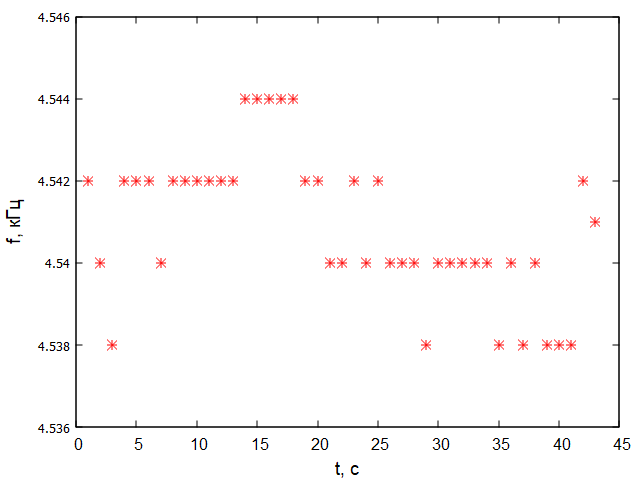
\includegraphics[width=0.8\textwidth]{graph1}
\caption{Зависимость результатов наблюдений от времени}
\label{fig:graph1}
\end{figure}

На рис.~\ref{fig:graph2} представлено распределение результатов наблюдений на числовой оси.
\begin{figure}[H]
\centering
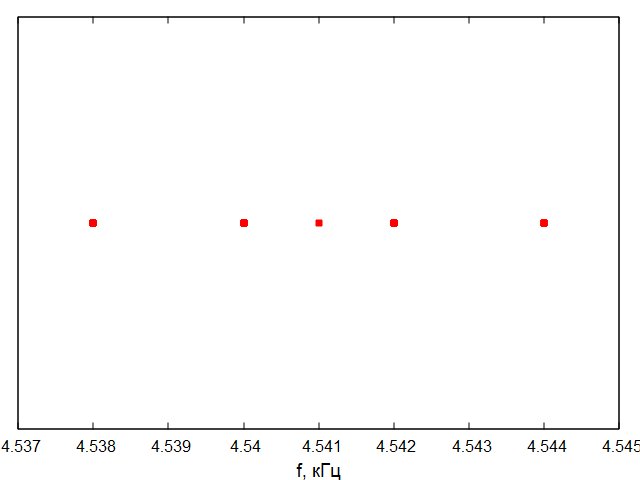
\includegraphics[width=0.8\textwidth]{graph2}
\caption{Распределение результатов наблюдений на числовой оси}
\label{fig:graph2}
\end{figure}
\begin{center}
\begin{table}[H]
\centering
\label{tabl:3}
\caption{Таблица распределения результатов}
\begin{tabular}{|c|c|c|c|c|}
\hline
\begin{minipage}{2cm}
    Номер интервала
\end{minipage}&
\begin{minipage}{3cm}
    Границы интервалов
\end{minipage} &
\begin{minipage}{5cm}
    Число случаев($\Delta n$), когда результат наблюдения попадает в данный интервал
\end{minipage} &
\begin{minipage}{5cm}
    Доля (часть) полного числа результатов, попадающих в этот интервал $\delta n=\frac{\Delta n}{n}$
\end{minipage}\\
\hline
1 &  [4.538,4.540)  &  7 & 0.16 \\
2 &  [4.540,4.542)  &  16 & 0.37 \\
3 &  [4.542,4.544)  &  15 & 0.35 \\
4 &  [4.544,4.546)  &  5 & 0.12 \\
\hline
\end{tabular}
\end{table}
\end{center}\\

\begin{figure}[H]
\centering
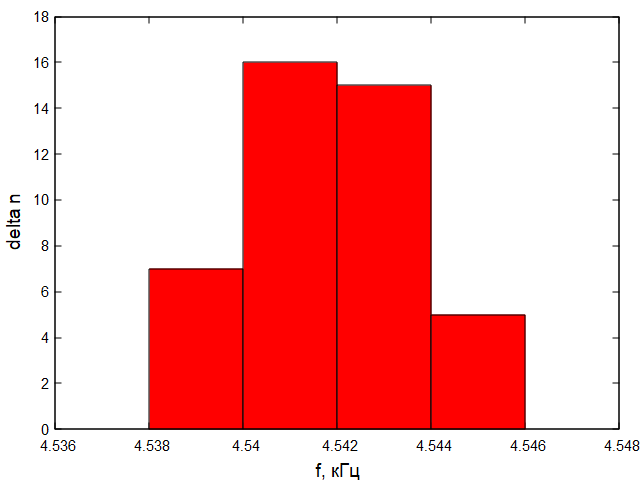
\includegraphics[width=1.0\textwidth]{gist}
\caption{Распределение результатов наблюдений: гистрограмма}
\label{fig:gist}
\end{figure}
\begin{figure}[H]
\centering
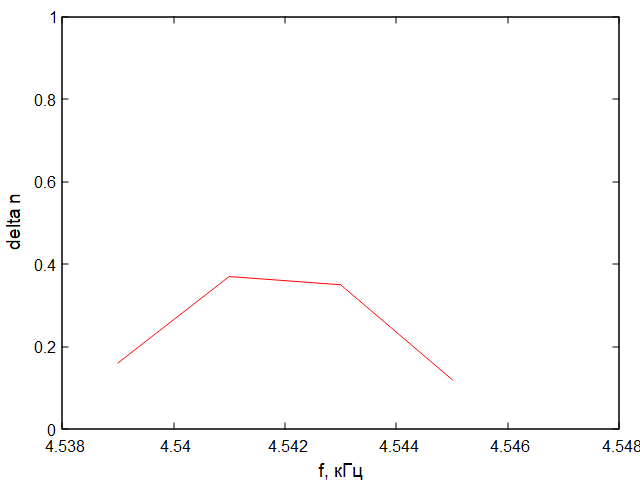
\includegraphics[width=0.8\textwidth]{graph3}
\caption{Распределение результатов наблюдений: график}
\label{fig:graph3}
\end{figure}\\
Были высчитаны следующие значения искомых величин:\\
Дисперсия: $\sigma=0.001813$ кГц\\
Средняя квадратичная погрешность среднего: $\sigma_f$=0.0002764 кГц\\
Так как случайная и системная погрешность одного порядка, применяем формулу:
\begin{equation}
    \sigma_{сумм}=\sqrt{(\frac{\Delta f_{прибора}}{3})^2+\sigma_f^2}
\end{equation}
\\
$\sigma_{сумм}=0.0004336$ кГц\\
Окончательный ответ: $f=4.541\pm0.0004336$ кГц\\
\section{Выводы}
В ходе выполнения данной лабораторной работы были освоены методики проведения многократных измерений частоты на измерительном приборе (частотомере ЧЗ-32). В процессе исследования были получены экспериментальные данные, которые подверглись статистической обработке. В частности, был проведён анализ данных, включающий построение таблиц распределения, графиков и гистограмм.

Кроме того, были рассчитаны основные статистические параметры, такие как дисперсия и средняя квадратичная погрешность среднего значения. Проведённый анализ способствовал углублению понимания природы случайных и систематических погрешностей, а также методов их учета при обработке экспериментальных данных. Полученные навыки могут быть применены для повышения точности измерений в дальнейших исследованиях.


\begin{thebibliography}{9}

%ссылка на репозиторий с исходныим кодом отчета и всех расчетных программ 
\bibitem{repo}
\url{https://github.com/st117207/Workshop1}  (дата обращения: 23.03.2024) 


\end{thebibliography}

